
% !TeX spellcheck = en_US
\documentclass[12pt, onecolumn]{article}

\usepackage{graphicx}

%opening
\title{Advanced Machine Learning - Assignment 5}
\author{Pranav Kasela \\$846965$}
\date{}
\begin{document}

\maketitle
\section*{Introduction}
The objective of this assignment is to use the SMBO models to find the hyperparameters of a Multi Layer Perceptron which maximizes the accuracy on a 10 folds cv.
The language used in this assignment is python with the SMAC package for the Hyperparameter optimization and Sklearn for the MLPerceptron.
Actually there is another easier package based on SMAC called `auto-sklearn', but in this assignment the basic SMAC package was used.
The dataset has 9 features and 1 target, the 9 features are apparently numeric, but the documentation explains that the variable V1 is the Season, which assumes the following values: $-1$:`winter', $-0.33$:`spring', $0.33$:`summer', $1.0$:`fall', since they are cyclic variable it cannot be considered completely correct to use ordered variable from $-1$ to $+1$, thus a one hot encoding is performed, another variable which cannot be considered equidistantly ordered is the V7 (Frequency of alcohol consumption), V7 assumes the following 5 values: $0.2$:`several times a day', $0.4$:`every day',$0.6$:`several times a week',  $0.8$:`once a week',$1.0$:`hardly ever never', a one hot encoding is also performed in this case.\\
This is the only basic preprocessing done on the data, the other values were accepted as numeric since they had mostly 2 or 3 classes or were already normalized.

\section*{SMAC}
The next step was to create a ``Wrapper'' around the SMAC package, just for our task (so it won't generalize well to other problems), this made the code easier for all the exercise.
The wrapper is named ``optimizer'' and it takes in input the surrogate model name (`rf', `gp') and will create SMAC4BO for the `gp' model and SMAC4HPO for the `rf' model, configuration space object containing information regarding, objective function which needs to be minimized, acquisition function name which can be `EI', `LCB' or `PI', number of iterations, initial points and an eventual seed.\\
The optimizer function creates every object necessary for SMAC: Scenario, AcquisionFunction, SMAC Objects etc., the code is commented in a very detailed way\footnote{Well surely better than the SMAC documentation.} so how the function works will not be explained here, the optimizer function return an optimized SMAC object with it's history.
The function uses RandomConfigurations to create the initial design, and its seed is the same as the SMAC object, so all the SMAC models with the same number of initial point will have the same performance on the initial points, and since a seed (123456789) is fixed for most of the randomness for reproducibility, so the model can be considered deterministic.
The objective function in SMAC can only be minimized so instead of weighted accuracy, $1 -$ weighted accuracy is used.
\section*{First Exercise}
For the First configuration a Configuration Space is created and it consists of two parameters the `learning\_rate\_init' with range between $0.01$ and $0.1$ and `momentum'  with range between $0.1$ and $0.9$, the metric used is an weighted accuracy, the weights of each class are the relative frequency of the other class, so the class `Normal' has a weight of $0.12$ and the class `Altered' (the rare one) has a weight of $0.88$, this choice tackles the class imbalance problem with such a low number of data which, since such small number of data makes the oversampling technique somehow problematic.\\
The `GP' surrogate model (SMAC4BO) is chosen for this part, and the acquisition functions `EI', `LCB' and `PI' are used with $5$ initial points, and the iterations are set to $25 (20 + 5$ initial$)$.
While for the GridSearch evenly distributed points are taken from the Configuration Domains (5 for each parameter), and RadomSearch searches random points by itself.
The MultiLayer perceptron classifier has two hidden layers with 4 and 2 neurons respectively and all the other configuration are the default one, except for the seed which is fixed to have consistent results. 
In the table \ref{tab:Ex1_res} are the result of the different acquisition function and models\footnote{The time values might differ a little in different runs because of the usual small randomnesses in the execution time, while the score should be consistent thanks to the seed.}.
Even though SMAC minimized the error, the weighted accuracy is used for the scores and plots to make them more intuitive.

\begin{table}[!h]
  \centering
  \begin{tabular}{ |c|c|c|c|c|c| } 
    \hline
    Acquisitions/Models$\to$ & LCB  & EI & PI & Random & Grid \\
    \hline
    Time(seconds) & 85.97 & 95.13 & 90.30 & 7.11 & 7.24\\
    \hline
    Score(weighted accuracy) & 0.582 & 0.580 & 0.580 & 0.580 & 0.544\\ 
    \hline
  \end{tabular}
  \caption{Results of the First Exercise}
  \label{tab:Ex1_res}
\end{table}

\begin{figure}[!h]
  \centering
  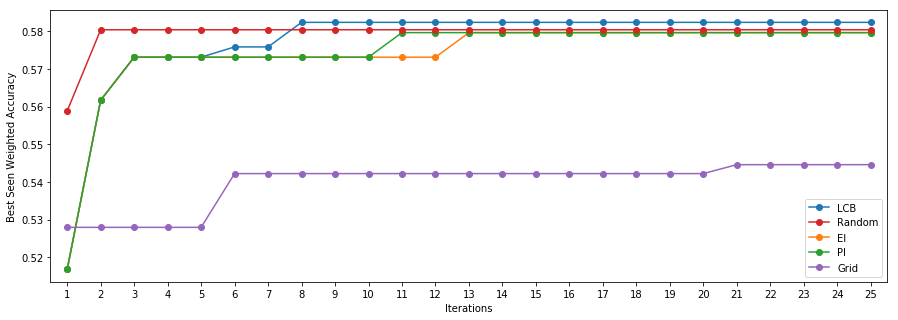
\includegraphics[width=\linewidth, height=5cm]{imgs/first.png}
  \caption{Plot of the result of the First Exercise}
  \label{fig:first}
\end{figure}
From the Table \ref{tab:Ex1_res} and Figure \ref{fig:first}, the best performance is obtained by the GP model with LCB as an acquisition function followed by the RandomSearch, which was fortunate enough to find the it's best configuration at the second iteration, the GP model with EI and PI have the same result and their score is very similar to the RandomSearch (it only differs of $0.0008$), while the worst performance is obtained by the GridSearch.
In the Figure \ref{fig:first} all the GP model have the same starting point while Grid and Randomized Search starts at different initial points.
The best configuration found is with a learning rate of $0.06690282$ and a momentum $0.20195706$ and in the Table \ref{tab:best_1} its performance on a 10-CV is reported.
\begin{table}[!h]
  \centering
  \begin{tabular}{ |c|c|c|c|c|c| } 
    \hline
    Metrics& F1 & Precision & Recall & F1 Macro & Accuracy\\
    \hline
    Score& 0.173 & 0.133 & 0.250 & 0.536 & 0.823\\
    \hline
  \end{tabular}
  \caption{Results of 10-CV of the Best Configuration for the First Exercise}
  \label{tab:best_1}
\end{table}

\section*{Second Exercise}
The surrogate model is changed to the RandomForest (SMAC4HPO).
Two more hyperparameters are added to the configuration space, the number of neurons of the first and second hidden layer, both with a range between $1$ and $5$, $10$ random initial points are chosen and the number of iteration is increased to $110 (100 + 10$ initial$)$.
The Random and Grid models are used too, in the latter cases the two configurations for the hidden layer size is merged into a single configuration called hidden layer size and it is a tuple of 2 numbers ranging both from 1 to 5.
While for the Random configuration obtaining $110$ iterations is easy, for the Grid Search 5 parameters from each configuration is chosen (5 for the learning rate, 5 for the momentum and 5 for the hidden layer sizes) obtaining 125 iterations, for the plot only the last 110 iterations are considered (just to make sure each algorithm has the same length for aesthetics).   
\begin{table}[!h]
  \centering
  \begin{tabular}{ |c|c|c|c|c|c| } 
    \hline
    Acquisitions/Models$\to$ & LCB  & EI & PI & Random & Grid \\
    \hline
    Time(seconds) & 210.00 & 210.06 & 213.81 & 24.21 & 23.90\\
    \hline
    Score(weighted accuracy) & 0.601 & 0.645 & 0.601 & 0.614 & 0.594\\ 
    \hline
  \end{tabular}
  \caption{Results of the Second Exercise}
  \label{tab:Ex2_res}
\end{table}

\begin{figure}[!h]
  \centering
  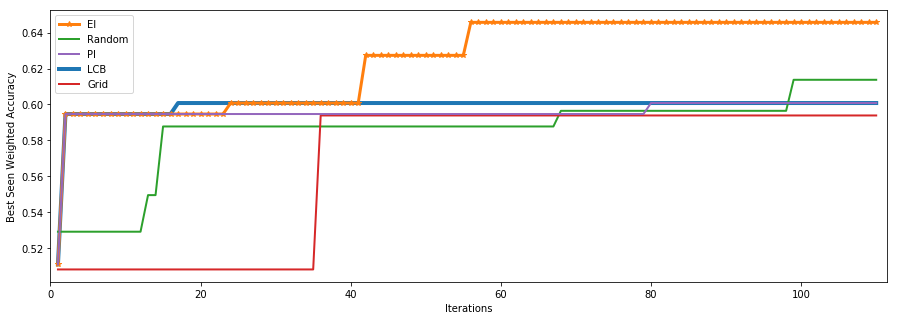
\includegraphics[width=\linewidth, height=5cm]{imgs/second.png}
  \caption{Plot of the result of the Second Exercise}
  \label{fig:second}
\end{figure}

From the Table \ref{tab:Ex2_res} and Figure \ref{fig:second} the best algorithm is the RandomForest with EI as acquisition function, improving the weighted accuracy from 0.58 (of the first exercise) to 0.645 with a learning rate of 0.01269289 and momentum of 0.73176491 and with 2 neurons in both layers, in Table \ref{tab:best_2}, it's performance on a 10-CV with other metrics is reported as well, the metric of out interest accuracy is now $0.911$, which is better than the zeroRule model\footnote{Trying to maximize the accuracy the optimizer converges to a ML model following a ZeroRule.}.
This result should not be surprising since it is known that EI is able to explore and still be able to exploit the information it has.
The LCB can be expected to fall in a local minima(maxima), but also the LCB was unable to find a better solution for a long number of iterations.\\
The Random and Grid Search model given more iteration outperforms the models in the First Exercise but requires less time, which is due to the fact that the points in Grid and Search does not depend from other chosen points, thus the calculation can be parallelized completely, in this case the computation was done on a 8 core computer, while the SMBO model needs to wait for the computation of a single configuration to decide the next one, there is an option to parallelize different algorithm in a cluster using `shared\_model' option in scenario Object of SMAC, an algorithm doesn't need to recompute the result of a a configuration that has already been tested on a different algorithm on another machine of the cluster, so using SMAC not in cluster is not really beneficial (for the parallelization). 
\begin{table}[!h]
  \centering
  \begin{tabular}{ |c|c|c|c|c|c| } 
    \hline
    Metrics& F1 & Precision & Recall & F1 Macro & Accuracy\\
    \hline
    Score& 0.300 & 0.300 & 0.300 & 0.626 & 0.911\\
    \hline
  \end{tabular}
  \caption{Results of 10-CV of the Best Configuration for the Second Exercise}
  \label{tab:best_2}
\end{table}

\section*{Conclusions}
% time of algorithm (GP is a lot slower than RF 3-4x)
One of things than can be noticed using GP as a surrogate model on the second exercise is that GP is about $5\times$ slower than the RF in this case taking nearly 1044 seconds while RF took only about $210$ seconds.\\
% why chose the new metric
% what happens if we use always accuracy <- plot of second_accuracy
The choice of a different metric than the one asked by the assignment is, as already mentioned, due to the class imbalance problem, but another motive is the fact that minimizing the requested metric `accuracy' with SMBO always made SMBO models to converge to the ZeroRule model, and being to be unable to find a better point of convergence (See Figure \ref{fig:second_acc}), some of the reasons are the lack of sufficient data and such a big number of folds in the cross validation, in fact, in each fold the model has at most 1 or 2 elements of the rare class in the test set, if it makes an error on that one the ML model has no more chance on improving its result, while using the weighted accuracy, more weight is given to the rare element, so the MLP is more attentive to that class, but it has the advantage that it does not neglect the non rare class.    
\begin{figure}[!h]
  \centering
  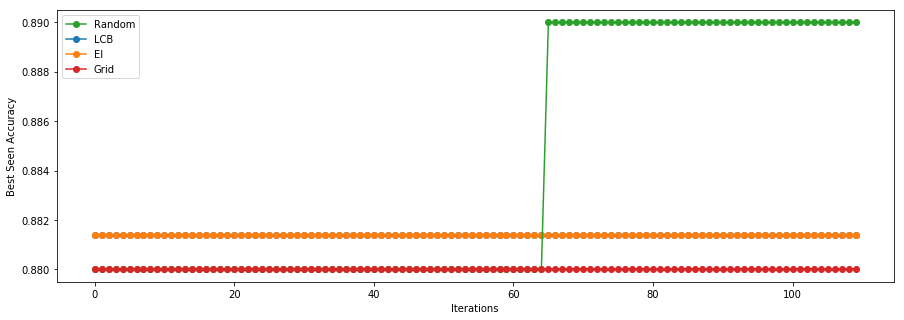
\includegraphics[width=\linewidth, height=5cm]{imgs/second_comparision_accuracy.png}
  \caption{Plot of result with accuracy as measure}
  \label{fig:second_acc}
\end{figure}
% does new metric improve the pure accuracy?
From the results of the second exercise it is clear that improving the model on weighted accuracy it a better choice, as it improves a lot also the accuracy, which was the objective of this assignment.
In the first exercise the model is not able to achieve a better result, due to less parameters that were being optimized and the low number of iterations.\\
The Grid Search is always outperformed by the other models, while surprisingly (or rather randomically) the Random Search has proved to be a good model, being able to obtain decent performances in both exercises (it is the second best model on both exercises), this was a simple case with a low dimensional hyperparameter space, but on more complex models the RandomSearch might have less chance to outperform Bayesian Models.
While the GridSearch doesn't scale well with the high dimensional spaces, the power of RandomSearch is to able to parallelize completely it's computation while it's randomness can be controlled in certain way using some more sophisticated sampling techniques for example the Quasi-Random models to match a more uniform distribution (Sobol, Latin Hypercube).
In this simple optimization problem the RandomSearch was able to complete the same number of configurations in $10\times$ less time, while using just one machine with 8 cores, while to parallelize a SMBO model with Bayesian Optimization with the methodologies used means executing more algorithms, for example using different surrogate models with different acquisition functions, in parallel which shares the Machine Learning Model behavior history in a shared memory.\\
A great way could be using RandomSearch with SMBO (in parallel), and use also the results of RandomSearch to help the SMBO models, this way there more information is given to the SMBO model and there is also a chance that the RandomSearch might find a better Minima than the one SMBO is trying to converge to.
% update the time is the tables

\end{document}